% !TEX root = ../main.tex

\subsection{MNIST data imbalance experiments} 

We use the standard MNIST handwritten digit classification dataset and subsample the dataset to
generate a class imbalance binary classification  task. We select a total of 5,000 images of size
28$\times$28 on class 4 and 9, where 9 dominates the training data distribution. We train a standard
LeNet on this task and we compare our method with a suite of commonly used tricks for class
imbalance: 1) \textsc{Proportion} weights each example by the inverse frequency 2) \textsc{Resample}
samples a class-balanced mini-batch for each iteration 3) \textsc{Hard Mining} selects the highest
loss examples from the majority class and 4) \textsc{Random} is a random example weight baseline
that assigns weights based on a rectified Gaussian distribution:
\begin{equation}
w_i^{\text{rnd}} = \frac{\max(z_i, 0)}{\sum_i \max(z_i, 0)},
\label{eq:randomwts}
\end{equation}
where $z_i \sim \mathcal{N}(0, 1)$.
To make sure that our method does
not have the privilege of training on more data, we split the balanced validation set of 10 images
directly from the training set. The network is trained with SGD with a learning rate of 1e-3 and
mini-batch size of 100 for a total of 8,000 steps.

Figure~\ref{fig:mnist_imba} plots the test error rate across various imbalance ratios averaged from
10 runs with random splits. Note that our method significantly outperforms all the baselines. With
class imbalance ratio of 200:1, our method only reports a small increase of error rate around 2\%,
whereas other methods suffer terribly under this setting. Compared with resampling and hard negative
mining baselines, our approach does not throw away samples based on its class or training loss - as
long as a sample is helpful towards the validation loss, it will be included as a part of the
training loss.

% !TEX root = ../main.tex

\begin{figure}
\centering
\iflatexml
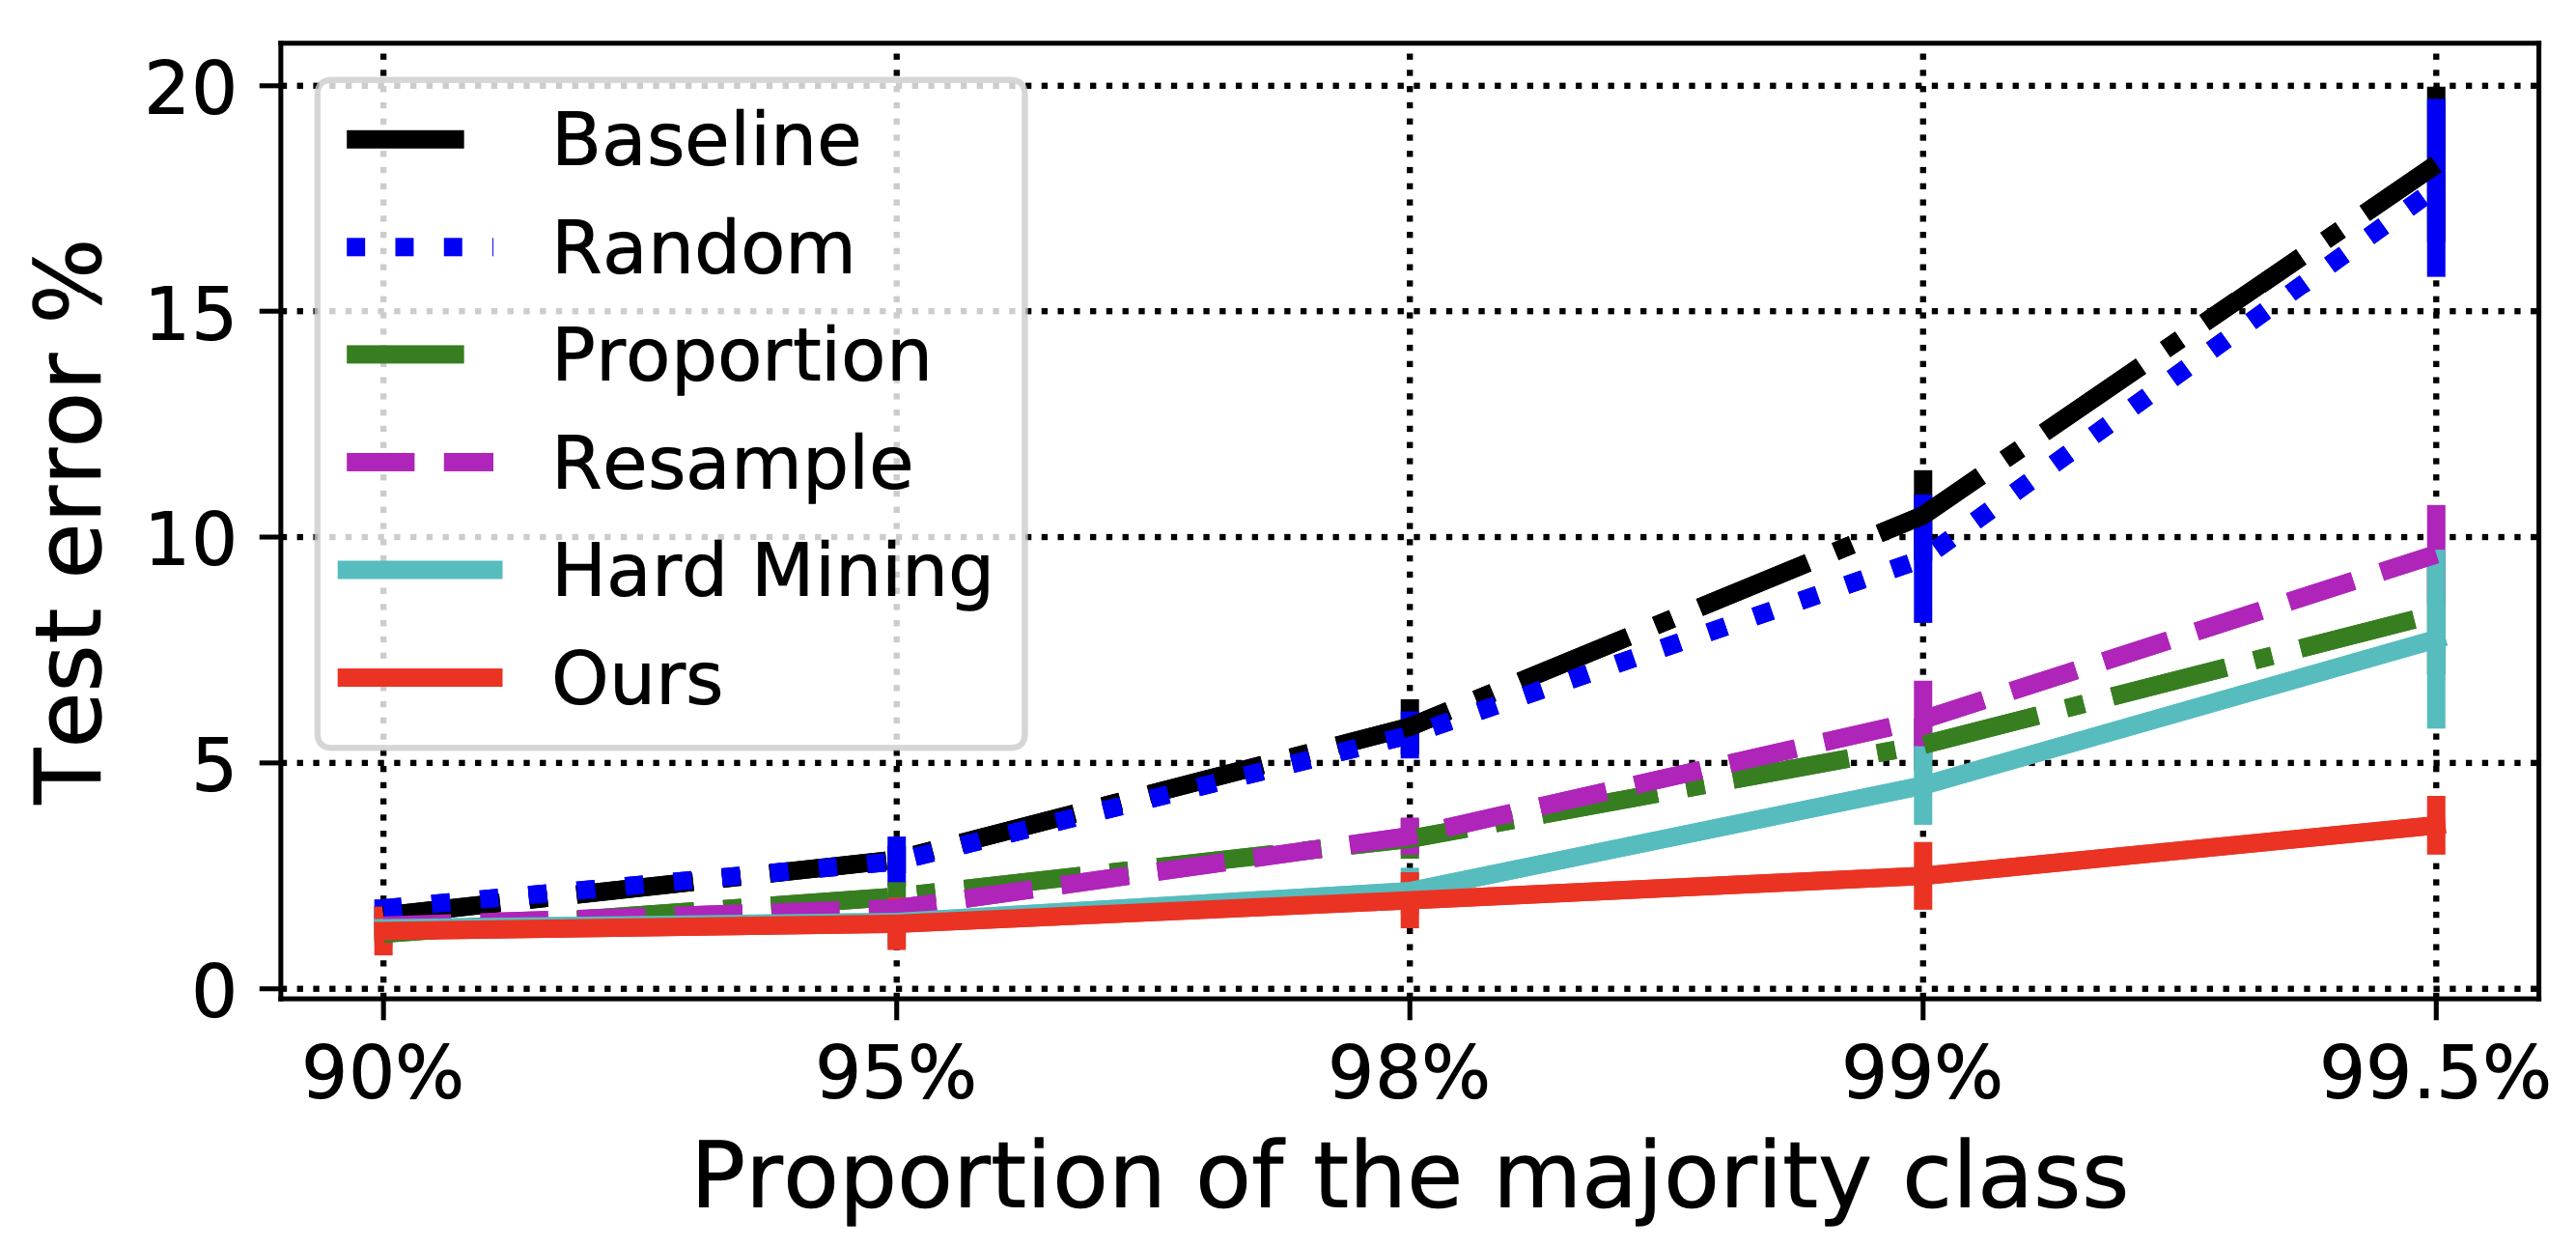
\includegraphics[width=6\columnwidth]{figures/mnist-imbalance.png}
\else
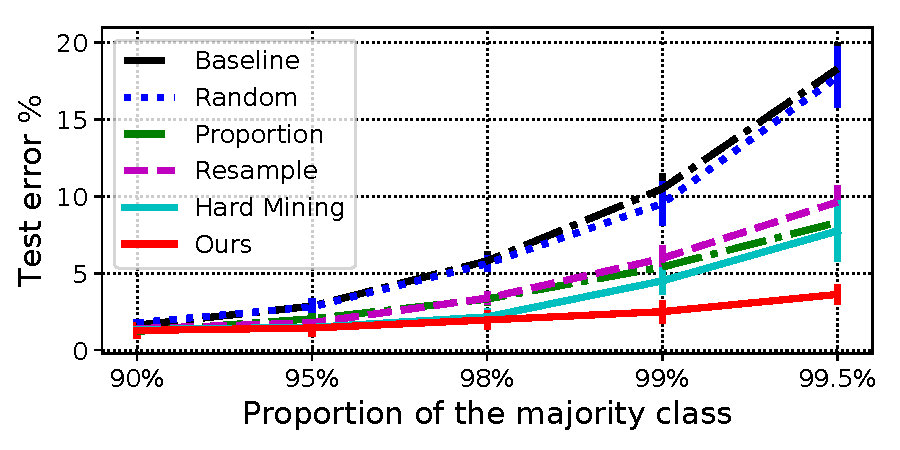
\includegraphics[width=0.9\columnwidth]{figures/mnist-imbalance.pdf}
\fi
\vspace{-0.1in}
\caption{MNIST 4-9 binary classification error using a LeNet on imbalanced classes. Our method uses a small balanced validation split of 10 examples.}
\label{fig:mnist_imba}
\end{figure}

